% Copyright 2004 by Till Tantau <tantau@users.sourceforge.net>.
%
% In principle, this file can be redistributed and/or modified under
% the terms of the GNU Public License, version 2.
%
% However, this file is supposed to be a template to be modified
% for your own needs. For this reason, if you use this file as a
% template and not specifically distribute it as part of a another
% package/program, I grant the extra permission to freely copy and
% modify this file as you see fit and even to delete this copyright
% notice. 

\documentclass{beamer}

% There are many different themes available for Beamer. A comprehensive
% list with examples is given here:
% http://deic.uab.es/~iblanes/beamer_gallery/index_by_theme.html
% You can uncomment the themes below if you would like to use a different
% one:
%\usetheme{AnnArbor}
%\usetheme{Antibes}
%\usetheme{Bergen}
%\usetheme{Berkeley}
%\usetheme{Berlin}
%\usetheme{Boadilla}
%\usetheme{boxes}
%\usetheme{CambridgeUS}
%\usetheme{Copenhagen}
%\usetheme{Darmstadt}
%\usetheme{default}
%\usetheme{Frankfurt}
%\usetheme{Goettingen}
%\usetheme{Hannover}
%\usetheme{Ilmenau}
%\usetheme{JuanLesPins}
%\usetheme{Luebeck}
\usetheme{Madrid}
%\usetheme{Malmoe}
%\usetheme{Marburg}
%\usetheme{Montpellier}
%\usetheme{PaloAlto}
%\usetheme{Pittsburgh}
%\usetheme{Rochester}
%\usetheme{Singapore}
%\usetheme{Szeged}
%\usetheme{Warsaw}
\usepackage{subcaption}
\title{Face Detection using Deep Learning}

% A subtitle is optional and this may be deleted
%\subtitle{Optional Subtitle}

\author{Akshay Khadse \and Ashish Sukhwani \and Raghav Gupta \and Soumya Dutta}
% - Give the names in the same order as the appear in the paper.
% - Use the \inst{?} command only if the authors have different
%   affiliation.

\institute[IITB] % (optional, but mostly needed)
{
  Indian Institute of Technology\\
  Bombay
}
% - Use the \inst command only if there are several affiliations.
% - Keep it simple, no one is interested in your street address.

\date{\today}
% - Either use conference name or its abbreviation.
% - Not really informative to the audience, more for people (including
%   yourself) who are reading the slides online

%\subject{Theoretical Computer Science}
% This is only inserted into the PDF information catalog. Can be left
% out. 

% If you have a file called "university-logo-filename.xxx", where xxx
% is a graphic format that can be processed by latex or pdflatex,
% resp., then you can add a logo as follows:

% \pgfdeclareimage[height=0.5cm]{university-logo}{university-logo-filename}
% \logo{\pgfuseimage{university-logo}}

% Delete this, if you do not want the table of contents to pop up at
% the beginning of each subsection:
\AtBeginSubsection[]
{
  \begin{frame}<beamer>{Outline}
    \tableofcontents[currentsection,currentsubsection]
  \end{frame}
}

% Let's get started
\begin{document}

\begin{frame}
  \titlepage
\end{frame}

\begin{frame}{Outline}
  \tableofcontents
  % You might wish to add the option [pausesections]
\end{frame}

% Section and subsections will appear in the presentation overview
% and table of contents.
\section{Introduction}

\subsection{Face Detection as problem}
\begin{frame}{Face Detection as problem}
  \begin{itemize}
  \item Pictures: Convenient medium of expression \vspace{0.75cm}
  \item Retrieving and Organisation of large collection is a challenge\vspace{0.75cm}
  \item Well established techniques for geotagging and timestamping.\vspace{0.75cm}
  \item More contextual queries: An issue drawing increased attention\vspace{0.75cm}
  \item Eg: Photos taken with a particular person.
  \end{itemize}
\end{frame}
\subsection{Relevance and Motivation}
\begin{frame}{Relevance and Motivation}
  \begin{itemize}
  \item Faces: Not unique rigid object\vspace{0.5cm}
  \item Inter-personal variations due to identity, genetics etc\vspace{0.5cm}
  \item Intra-personal variations due to expressions, aging, facial hair etc\vspace{0.5cm}
  \item Active research since two decades have resulted in well established techniques\vspace{0.5cm}
  \item These methods fail to detect faces with different angle, partial faces.
  \end{itemize}
\end{frame}
\subsection{Motivation}

\section{Existing Methodologies}
\subsection{Haar Cascade}
\begin{frame}{Haar Cascade}
  \begin{itemize}
      \item Haar feature based Cascade Classifers
      \item Haar features are extracted from images
      \item Construct feature vector of each image
      \item Adaboost: Selecting from large Number of features
      \item Final Classifier: Weighted sum of individual classifier at each step
      \item Works very well for images with frontal faces
      \item Not satisfactory for images with other views, multiple faces
  \end{itemize}
\end{frame}

% Placing a * after \section means it will not show in the
% outline or table of contents.
\section{Method Described in paper}
\subsection{Preprocessing}
\begin{frame}{Preprocessing}
  \begin{itemize}
      \item Main paper referred \cite{paper} describesfinetuning of AlexNet for multiview face detection
      \item AFLW dataset: 21k images with 24k face annotations
      \item Randomly sampling sub windows of the images
      \item IOU with ground truth to increase number of examples
      \item IOU $> 50\%$: Positive example, IOU $< 30\%$: Negative example
      \item 200k positive examples, 20 million negative examples
      \item Image size $227\times227\times3$.
  \end{itemize}
\end{frame}
\subsection{Training}
\begin{frame}{Training}
  \begin{itemize}
      \item AlexNet: 5 Convolutional Layers, # Fully connected Layers
      \item Batch Size 128: 32 Positive examples, 96 Negative Examples
      \item Trained for 50K iterations
      \item Final detector can be using Region based or sliding window approach
      \item This method uses sliding window approach due to its less complexity
      %\item Original authors used caffe for implementation
      \item Paper describes comparison of this method with R-CNN
      \item AlexNet trained by reshaping output of fully connected layer for training SVM classier
      \item A bounding box regression unit was trained
      \item Both methods also trained on PASCAL VOC 2013 objects
  \end{itemize}
\end{frame}
\subsection{Results}
\begin{frame}{Results}
  \begin{itemize}
      \item Face trained AlexNet performs better than PASCAL VOC trained AlexNet
      \item Significant improvement of R-CNN due to bounding box regression
      \item Performance of RCNN not as good as previous method
      \item Reasons for inferior performance
      \begin{itemize}
        \item Selective search leading to missing out some of face regions.
        \item Imperfection in bounding box regression.
      \end{itemize}
  \end{itemize}
\end{frame}


\section{Our Methodology}
\subsection{Data Collection and Pre-processing}
\begin{frame}{Data Collection and Pre-processing}
  \begin{itemize}
      \item Same AFLW dataset used
      \item Dataset augmented in same way as described in \cite{paper}
      \item Total 24k positive and 120k negative
      \item Images reduced to $128\times128$
      \item All images converted to grayscale
  \end{itemize}
\end{frame}
\subsection{Network Architecture}
\begin{frame}{Network Architecture}
  \begin{itemize}
    \item CONV LAYER 1(Activation - ReLU Filter - $18\times18\times1\times60$ Bias - $60$ Stride - $1\times1$)
    \item MAXPOOL LAYER1(Filter - $2\times2$ Stride - $2\times2$)
    \item CONV LAYER 2(Activation - ReLU Filter - $12\times12\times60\times30$ Bias - $30$ Stride - $1\times1$)
    \item MAXPOOL LAYER2(Filter - $2\times2$ Stride - $2\times2$)
    \item CONV LAYER 3(Activation - ReLU Filter - $6\times6\times30\times15$ Bias - $15$ Stride - $1\times1$)
    \item MAXPOOL LAYER3(Filter - $2\times2$ Stride - $2\times2$)
    \item FC LAYER 1(Activation - ReLU Weights - $3840\times4096$ Bias - 4096)
    \item FC LAYER 2(Activation - ReLU Weights - $4096\times256$ Bias - 256)
    \item FC LAYER 3(Activation - Sigmoid Weights - $256\times1$ Bias - 4096)
  \end{itemize}
\end{frame}
\subsection{Training}
\begin{frame}{Training}
  \begin{itemize}
    \item Batch size 60, 50K iterations
    \item Originally Cross entropy with regularisation was used as cost
    \item Cost showed decreasing trend, accuracy finally setlled on 75\%.
    \item Weights at end of training were very small
    \item Modified cost function: Multiplying error on positive by a constant $\geqslant$ 3.5
    \item Training accuracy of $\geqslant$ 85\% was achieved
    \item Changing regularization parameter did not affect training accuracy
    \item 3 models with accuracies  88.3333\%, 91.6667\%, 94.2857\% were saved for testing.
  \end{itemize}
\end{frame}

\section{Results}
\begin{frame}{Results}
  \begin{figure}[h]
  \begin{subfigure}{\linewidth}
  \centering
  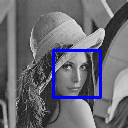
\includegraphics[width=.3\linewidth]{lenahaar.png}\hfill
  \caption{Haar Cascade Classifer for Image with single face}
  \end{subfigure}\par\medskip
  \begin{subfigure}{\linewidth}
  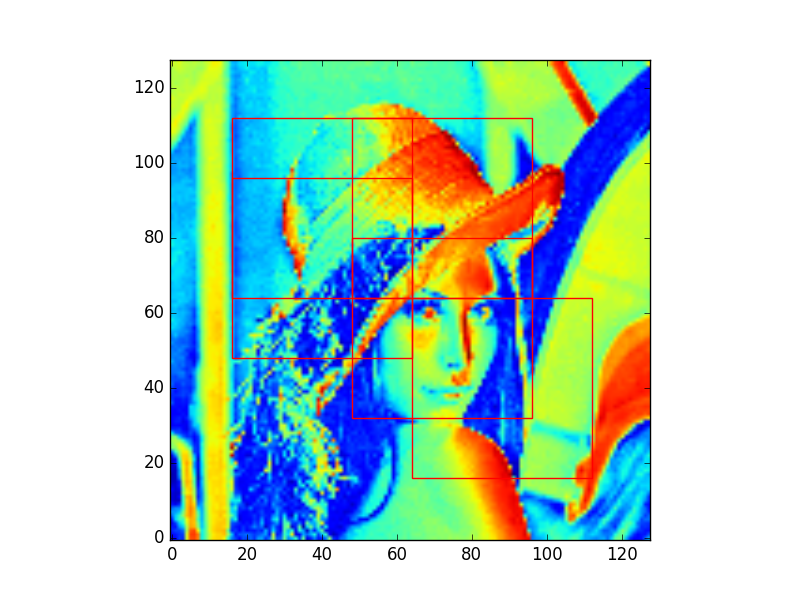
\includegraphics[width=.3\linewidth]{lena83.png}\hfill
  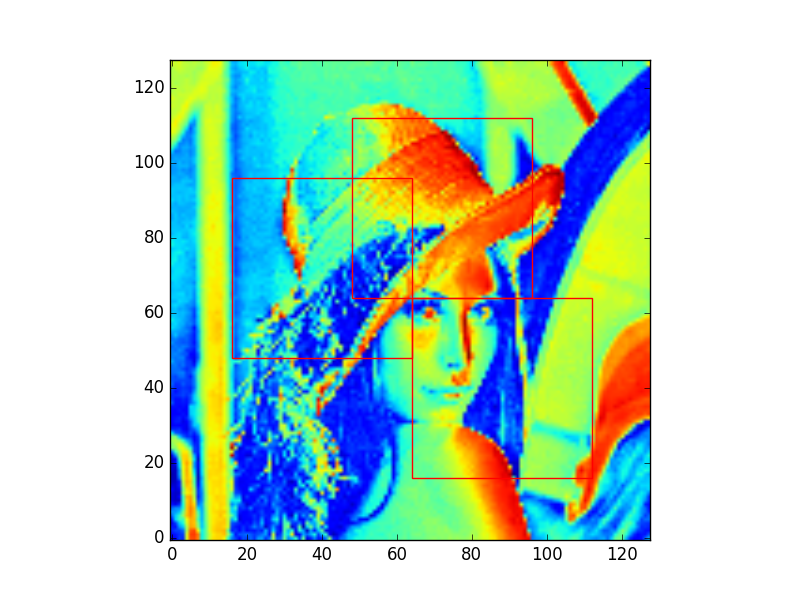
\includegraphics[width=.3\linewidth]{lena91.png}\hfill
  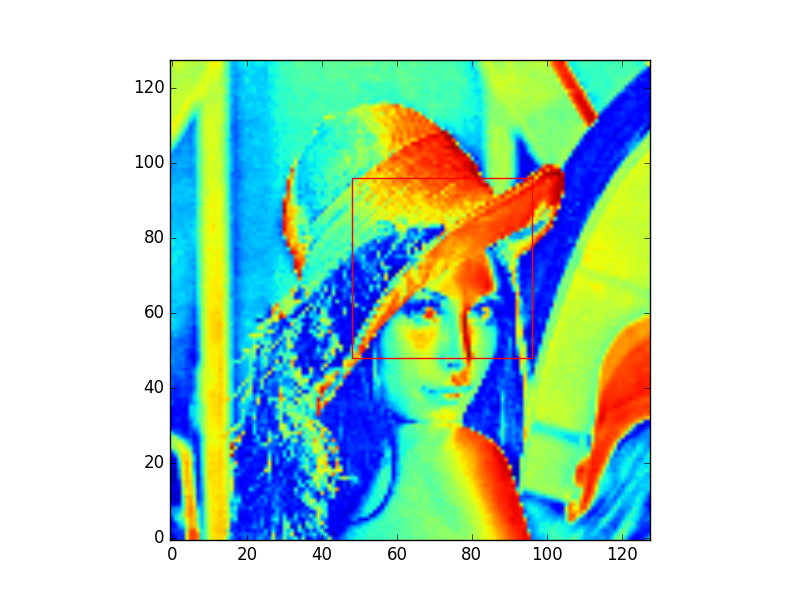
\includegraphics[width=.3\linewidth]{lena94.png}
  \caption{Our face detector performance-model 1 to 3 (left to right)}
  \end{subfigure}\par\medskip
  \caption{Number of faces is 1}
\end{figure}
\end{frame}
\begin{frame}{Results}
  \begin{figure}[h]
  \begin{subfigure}{\linewidth}
  \centering
  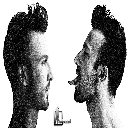
\includegraphics[width=.3\linewidth]{twohaar.png}\hfill
  \caption{Haar Cascade Classifer for Image with two faces}
  \end{subfigure}\par\medskip
  \begin{subfigure}{\linewidth}
  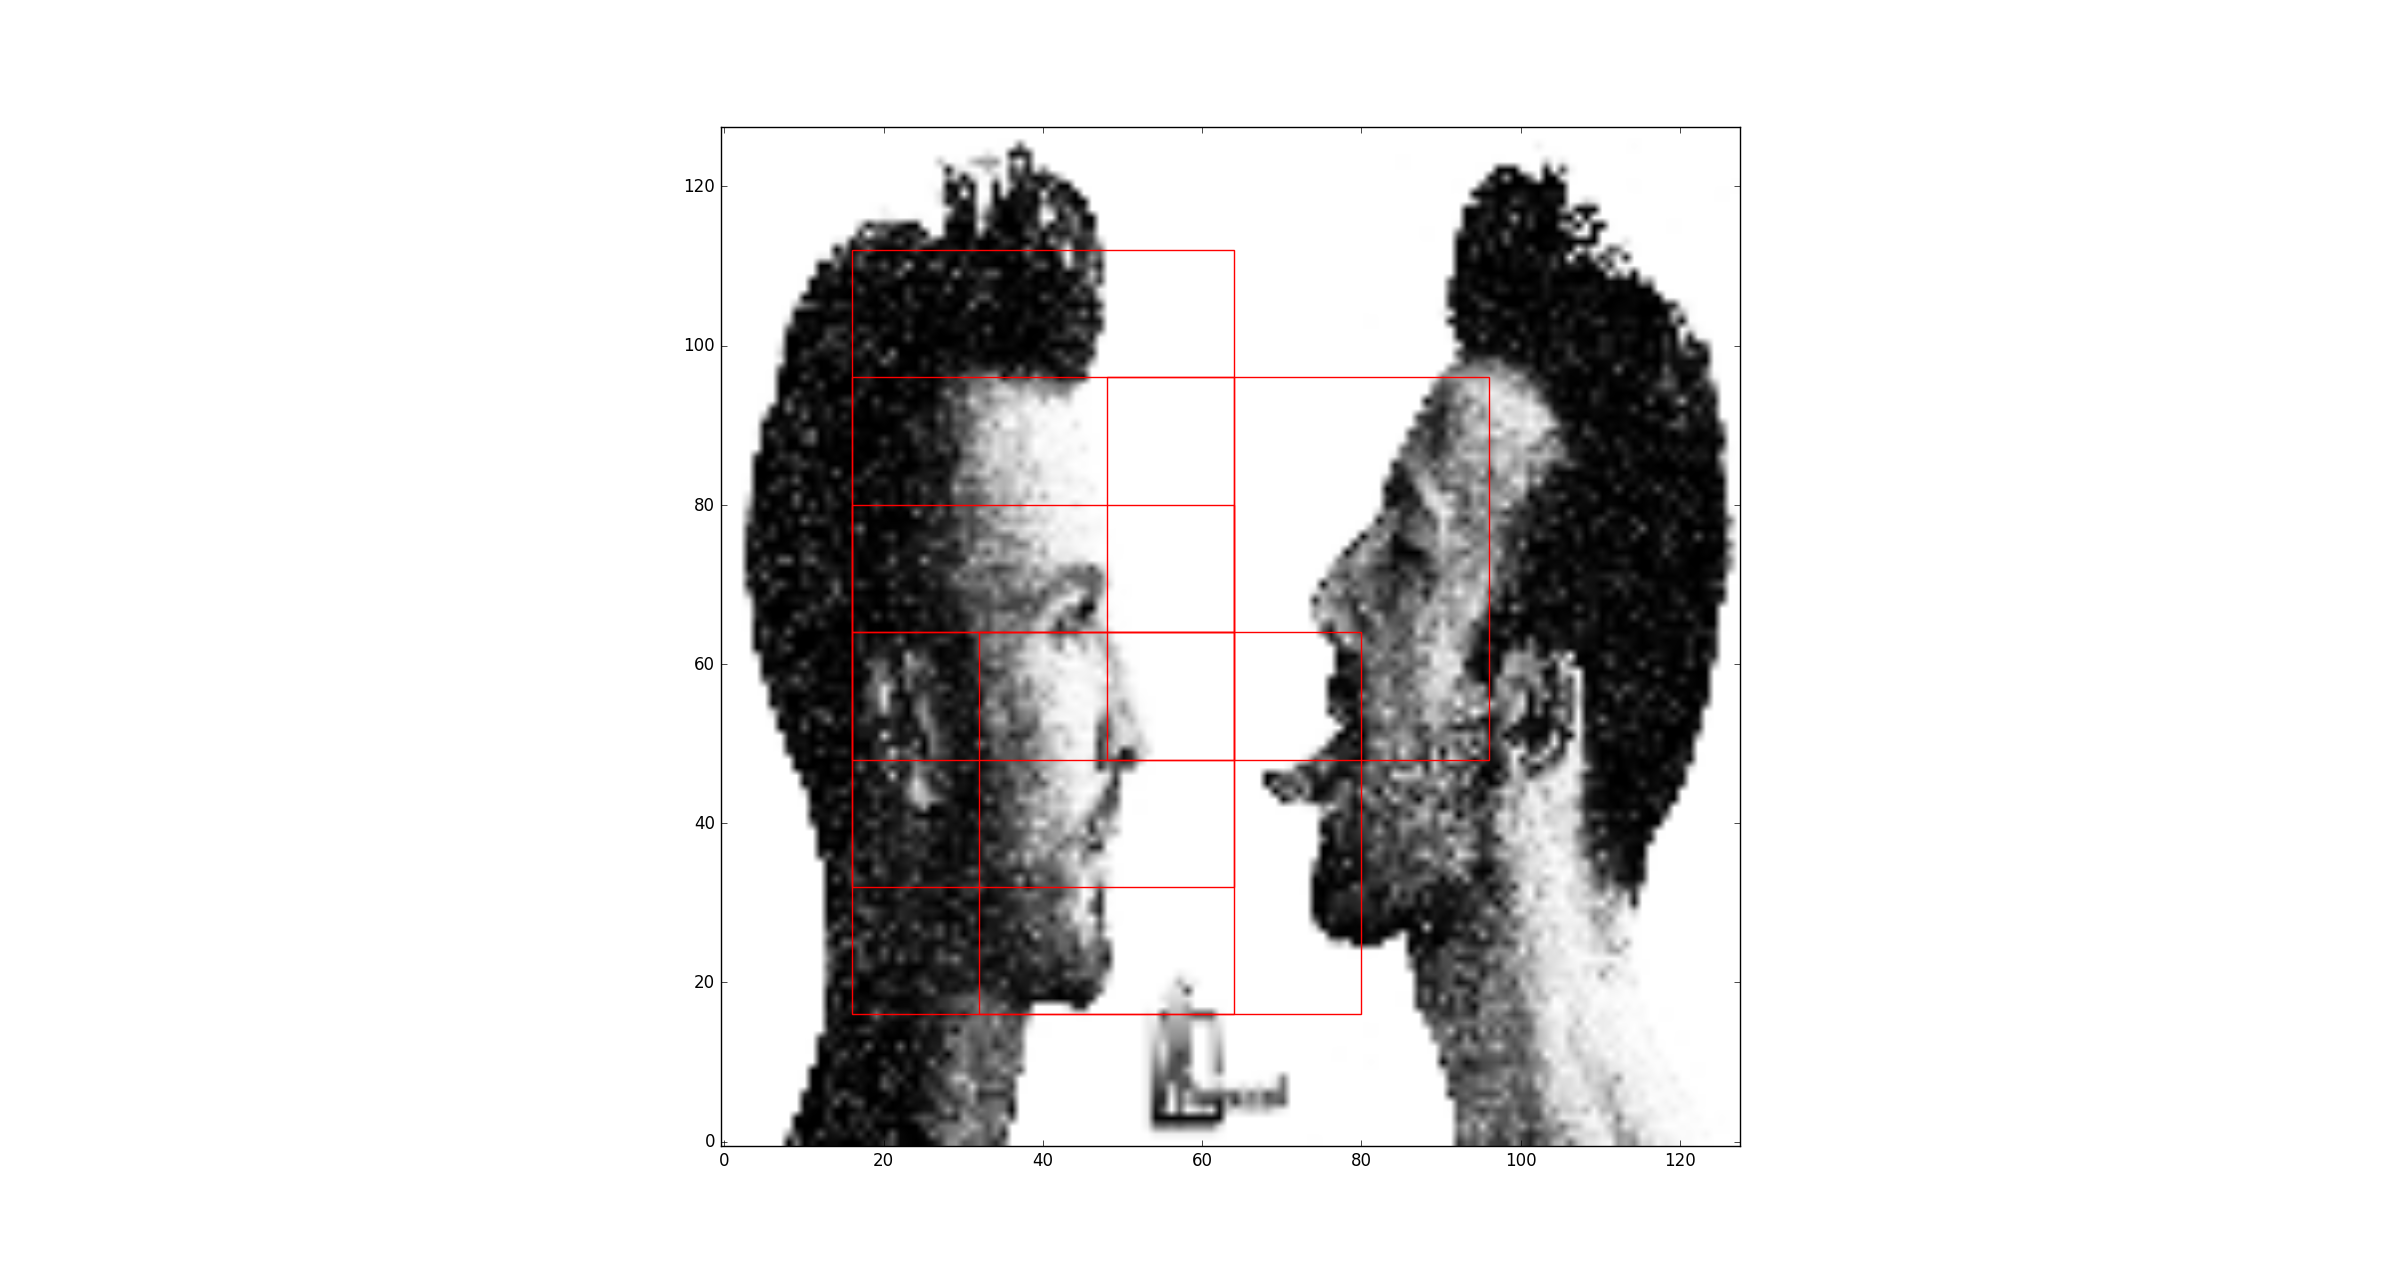
\includegraphics[width=.3\linewidth]{two83.png}\hfill
  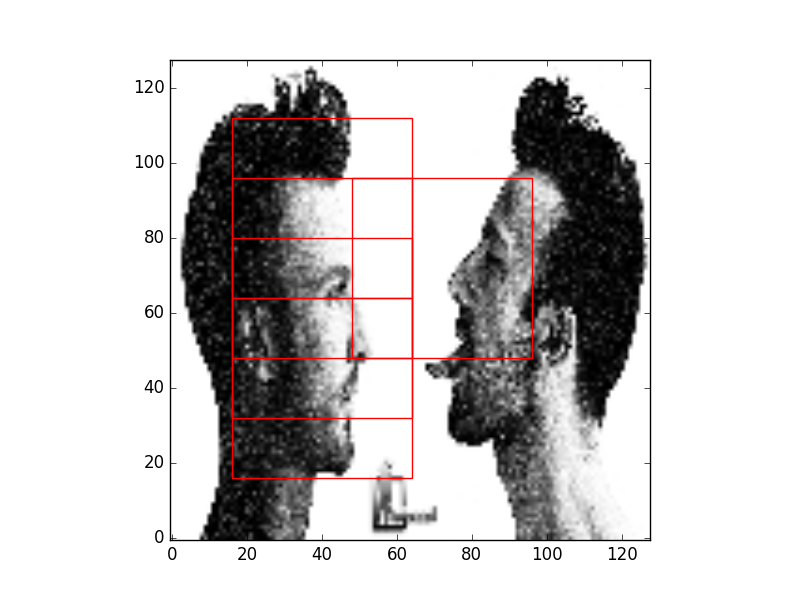
\includegraphics[width=.3\linewidth]{two91.png}\hfill
  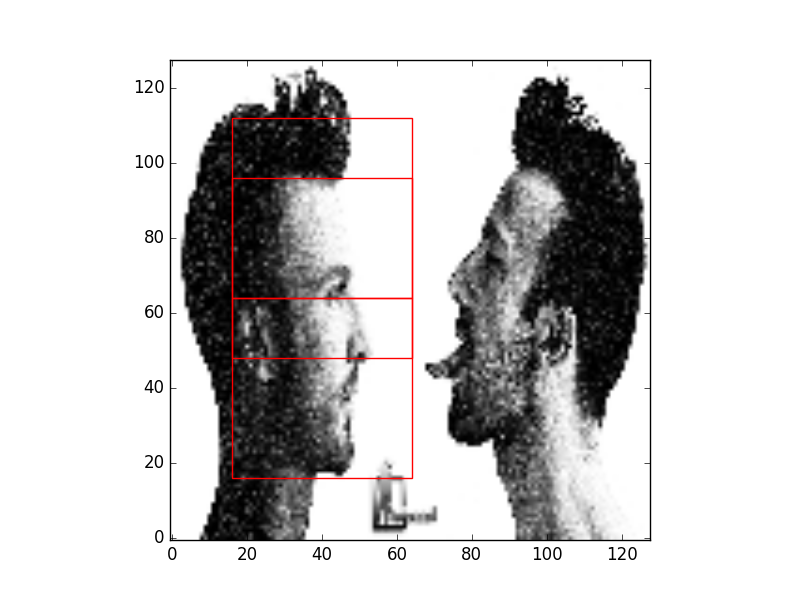
\includegraphics[width=.3\linewidth]{two94.png}
  \caption{Our face detector performance-model 1 to 3 (left to right)}
  \end{subfigure}\par\medskip
  \caption{Number of faces are 2}
\end{figure}
\end{frame}
\begin{frame}{Results}
\begin{figure}[h!]
  \begin{subfigure}{\linewidth}
  \centering
  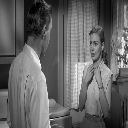
\includegraphics[width=.3\linewidth]{twomodhaar.png}\hfill
  \caption{Haar Cascade Classifer for Image with two faces}
  \end{subfigure}\par\medskip
  \begin{subfigure}{\linewidth}
  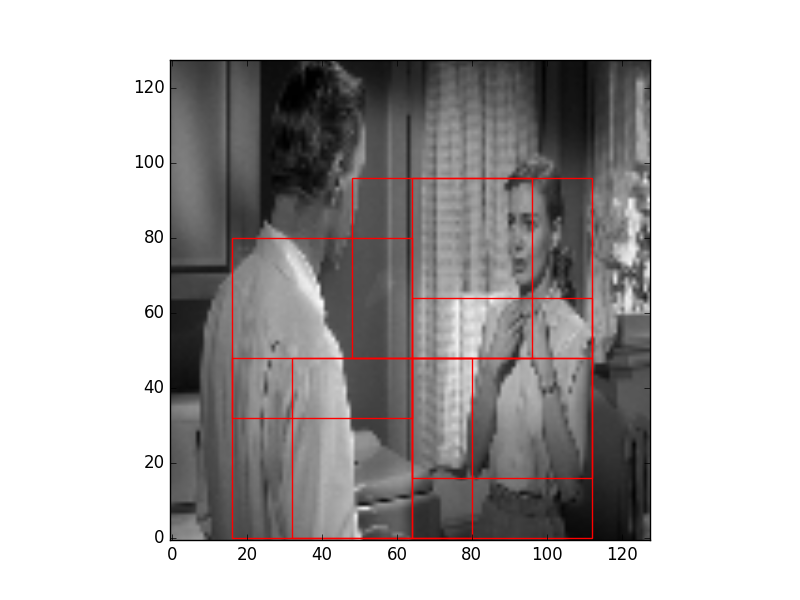
\includegraphics[width=.3\linewidth]{twomod83.png}\hfill
  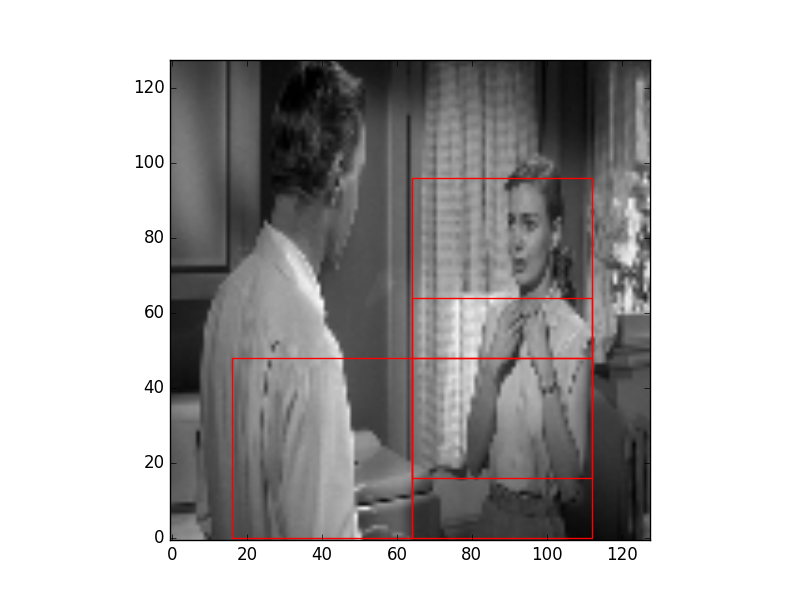
\includegraphics[width=.3\linewidth]{twomod91.png}\hfill
  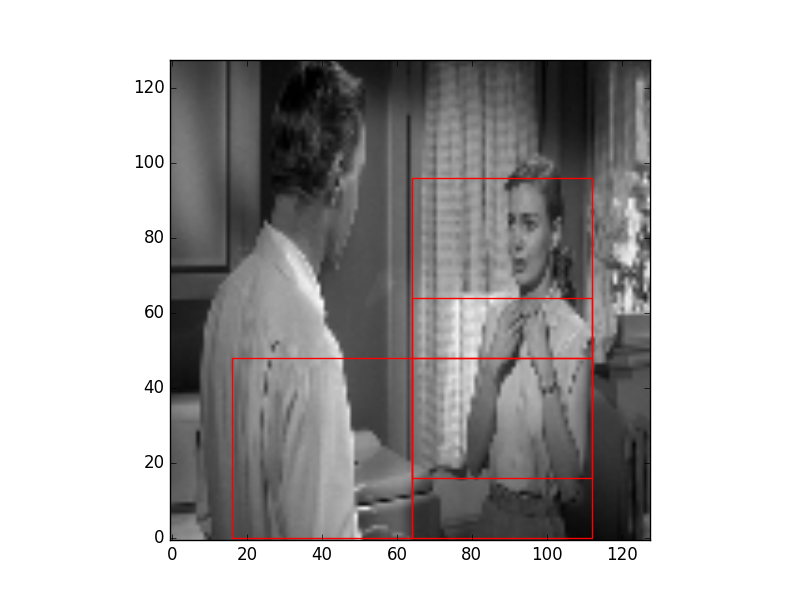
\includegraphics[width=.3\linewidth]{twomod94.png}
  \caption{Our face detector performance-model 1 to 3 (left to right)}
  \end{subfigure}\par\medskip
  \caption{Number of faces are 2}
  \end{figure}
\end{frame}
\begin{frame}{Results}
\begin{figure}[h!]
  \begin{subfigure}{\linewidth}
  \centering
  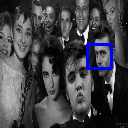
\includegraphics[width=.3\linewidth]{twitterhaar.png}\hfill
  \caption{Haar Cascade Classifer for Image with two faces}
  \end{subfigure}\par\medskip
  \begin{subfigure}{\linewidth}
  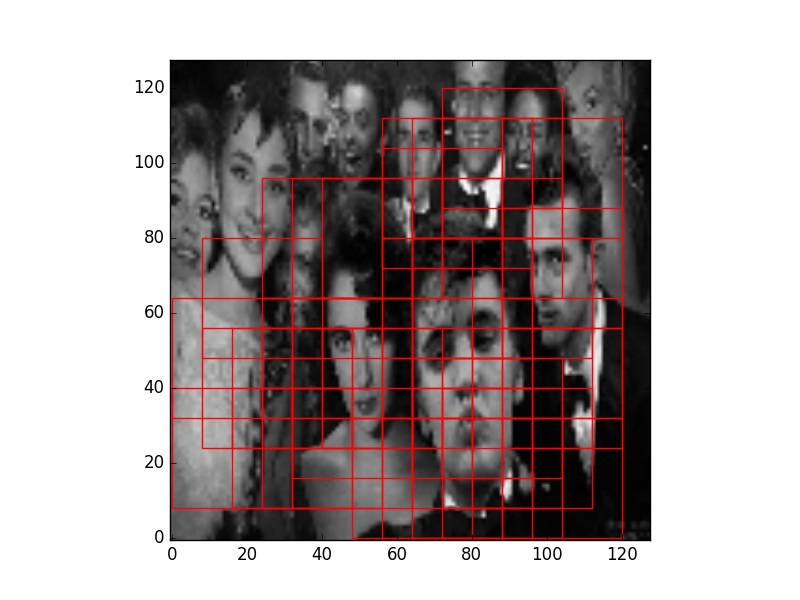
\includegraphics[width=.3\linewidth]{twitter83.png}\hfill
  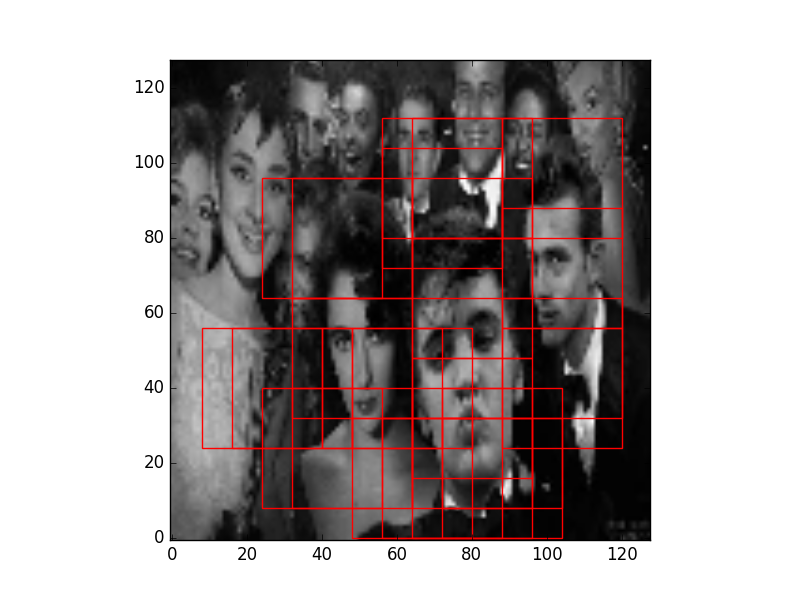
\includegraphics[width=.3\linewidth]{twitter91.png}\hfill
  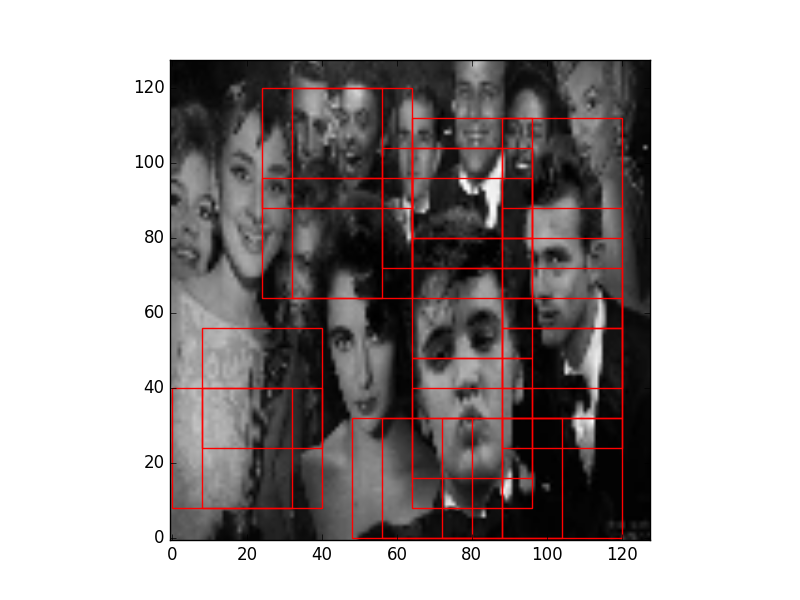
\includegraphics[width=.3\linewidth]{twitter94.png}
  \caption{Our face detector performance-model 1 to 3 (left to right)}
  \end{subfigure}\par\medskip
  \caption{Number of faces are $>$6}
\end{figure}
\end{frame}

\section{Conclusions}
\begin{frame}{Conclusions}
  \begin{itemize}
    \item A Deep Convolutional Neural Network was designed and using Tensorflow to detect faces from images
    \item A comparative study of this face detector was carried out against Haar cascade.
    \item Results significantly superior to the the Haar Cascade Classifier were achieved.
    \item Network is much simple than one described in paper\cite{paper}
    \item Many false positives are an issue.
  \end{itemize}
\end{frame}

\section{Timeline}
\begin{frame}{Timeline}
  \begin{itemize}
    \item Upto midterm-Collection and Pre-processing of data-initial architecture of the CNN 
    \item Experimented with different network architectures
    \item Changing the cost function to increase training accuracy
    \item Comparison of Haar Cascade Classifier and our face detector
    \item Tested the models on some test images
    \item Implemented PCA for face detection at a preliminary level.
  \end{itemize}
\end{frame}


\begin{frame}[allowframebreaks]
  \frametitle<presentation>{References}

  \begin{thebibliography}{99}
  \setlength{\itemsep}{0\parskip}
  \bibitem{viola}Jones, Michael, and Paul Viola. "Fast multi-view face detection." Mitsubishi Electric Research Lab TR-20003-96 3 (2003): 14.
  \bibitem{paper}Farfade, Sachin Sudhakar, Mohammad J. Saberian, and Li-Jia Li. "Multi-view face detection using deep convolutional neural networks." Proceedings of the 5th ACM on International Conference on Multimedia Retrieval. ACM, 2015.
  \bibitem{dataset}Zhang, Zhanpeng, et al. "Facial landmark detection by deep multi-task learning." European Conference on Computer Vision. Springer International Publishing, 2014.
  \end{thebibliography}
\end{frame}

\end{document}


